%% 
%% Copyright 2007-2024 Elsevier Ltd
%% 
%% This file is part of the 'Elsarticle Bundle'.
%% ---------------------------------------------
%% 
%% It may be distributed under the conditions of the LaTeX Project Public
%% License, either version 1.3 of this license or (at your option) any
%% later version.  The latest version of this license is in
%%    http://www.latex-project.org/lppl.txt
%% and version 1.3 or later is part of all distributions of LaTeX
%% version 1999/12/01 or later.
%% 
%% The list of all files belonging to the 'Elsarticle Bundle' is
%% given in the file `manifest.txt'.
%% 
%% Template article for Elsevier's document class `elsarticle'
%% with numbered style bibliographic references
%% SP 2008/03/01
%% $Id: elsarticle-template-num.tex 249 2024-04-06 10:51:24Z rishi $
%%
\documentclass[preprint,12pt]{elsarticle}

%% Use the option review to obtain double line spacing
%% \documentclass[authoryear,preprint,review,12pt]{elsarticle}

%% Use the options 1p,twocolumn; 3p; 3p,twocolumn; 5p; or 5p,twocolumn
%% for a journal layout:
%% \documentclass[final,1p,times]{elsarticle}
%% \documentclass[final,1p,times,twocolumn]{elsarticle}
%% \documentclass[final,3p,times]{elsarticle}
%% \documentclass[final,3p,times,twocolumn]{elsarticle}
%% \documentclass[final,5p,times]{elsarticle}
%% \documentclass[final,5p,times,twocolumn]{elsarticle}

%% For including figures, graphicx.sty has been loaded in
%% elsarticle.cls. If you prefer to use the old commands
%% please give \usepackage{epsfig}

%% The amssymb package provides various useful mathematical symbols
\usepackage{amssymb}
%% The amsmath package provides various useful equation environments.
\usepackage{amsmath}
%% The amsthm package provides extended theorem environments
%% \usepackage{amsthm}

%% The lineno packages adds line numbers. Start line numbering with
%% \begin{linenumbers}, end it with \end{linenumbers}. Or switch it on
%% for the whole article with \linenumbers.
%% \usepackage{lineno}

\journal{Computerized Medical Imaging and Graphics}

\begin{document}

\begin{frontmatter}

%% Title, authors and addresses

%% use the tnoteref command within \title for footnotes;
%% use the tnotetext command for theassociated footnote;
%% use the fnref command within \author or \affiliation for footnotes;
%% use the fntext command for theassociated footnote;
%% use the corref command within \author for corresponding author footnotes;
%% use the cortext command for theassociated footnote;
%% use the ead command for the email address,
%% and the form \ead[url] for the home page:
%% \title{Title\tnoteref{label1}}
%% \tnotetext[label1]{}
%% \author{Name\corref{cor1}\fnref{label2}}
%% \ead{email address}
%% \ead[url]{home page}
%% \fntext[label2]{}
%% \cortext[cor1]{}
%% \affiliation{organization={},
%%             addressline={},
%%             city={},
%%             postcode={},
%%             state={},
%%             country={}}
%% \fntext[label3]{}

\title{Optimizing Radiomic Feature Selection for Robust and Reproducible Binary Classification}

%% use optional labels to link authors explicitly to addresses:
%% \author[label1,label2]{}
%% \affiliation[label1]{organization={},
%%             addressline={},
%%             city={},
%%             postcode={},
%%             state={},
%%             country={}}
%%
%% \affiliation[label2]{organization={},
%%             addressline={},
%%             city={},
%%             postcode={},
%%             state={},
%%             country={}}

\author[FEEC]{Petra~Nemcekova}
\author[FEEC]{Jiri~Chmelik}
\author[FEEC]{Tomas~Vicar}
\author[UMC]{Mahsa~Mojtahedi}
\author[UMC]{Henk~A.~Marquering}
\author[FEEC]{Roman~Jakubicek} %% Author name

%% Author affiliation
\affiliation[FEEC]{organization={Department of Biomedical Engineering and Bioinformatics, Brno University of Technology},%Department and Organization
            addressline={Technická 3082/12}, 
            city={Brno},
            postcode={61200}, 
            state={Czech Republic},
            country={Czech Republic}}
\affiliation[UMC]{organization={Department of Biomedical Engineering and Physics, Amsterdam UMC Location AMC},%Department and Organization
            addressline={Meibergdreef 9}, 
            city={Amsterdam},
            postcode={1105 AZ}, 
            state={Netherlands},
            country={Netherlands}}
\cortext[cor1]{jakubicek@vut.cz}

%% Abstract
\begin{abstract}
%% Text of abstract does not exceed 250 words
% - 1 veta background (prečo je predikcia eTICI≥2B klinicky relevantná)
% - 1 veta gap (van Voorst 2023 = jedna kombinácia feature selection/klasifikátora, žiadne systematické porovnanie)
% - 1–2 vety metóda (rozsah faktoriálneho dizajnu: X feature-set × Y metód, CV + externá validácia, permutačný test)
% - 2–3 vety kľúčové výsledky (čísla AUC, štatistická signifikancia vs. chance)
% - 1 veta záver/implikácia
\end{abstract}

%%Graphical abstract
\begin{graphicalabstract}
%\includegraphics{grabs}
\end{graphicalabstract}

%% Keywords
\begin{keyword}
%% keywords here, in the form: keyword \sep keyword
brain stroke \sep thrombus \sep radiomics \sep CT
%% PACS codes here, in the form: \PACS code \sep code
87.19.xq \sep 87.57.Q
%% MSC codes here, in the form: \MSC code \sep code
%% or \MSC[2008] code \sep code (2000 is the default)

\end{keyword}

%%Research highlights
\begin{highlights} %% Highlights should consist of 3 to 5 bullet points, each a maximum of 85 characters, including spaces.
\item Research highlight 1 - Predictive Trained models
\item Research highlight 2 - Trained models freely available and repository
\item Research highlight 3 - Explore the influence of the method and dataset to prediction accuracy ?
\item Research highlight 4 - Explore the influence of segmentation size to prediction accuracy ?
\end{highlights}


\end{frontmatter}

%% Add \usepackage{lineno} before \begin{document} and uncomment 
%% following line to enable line numbers
% \usepackage{lineno}
% \linenumbers

%% main text
%%

%% Use \section commands to start a section
\section{Introduction}
\label{sec1}
% - Klinický kontext: EVT pri veľkocievnom uzávere, eTICI škála ako outcome, prečo je predikcia úspešnosti reperfúzie klinicky užitočná (voľba stratégie/zariadenia, informovanie pacienta/tímu, procedurálne plánovanie)
% - State of the art zameraný na: (a) radiomika trombu vo všeobecnosti, (b) konkrétne van Voorst et al. 2023 — čo urobili, aké AUC dosiahli pre eTICI≥2B (~0.52–0.56, teda blízko náhode) vs. pre mRS≤2 (~0.78–0.81), aký feature-selection použili (ICC≥0.75 filter, RF, žiadny ďalší výber príznakov)
% - Gap/limitácia predchádzajúcej práce: jedna pevná kombinácia feature-selection + klasifikátor; žiadne porovnanie granularity príznakov (voxel/distribution/global, whole vs. skeleton); žiadny permutačný test proti empirickému chance-baseline; žiadne overenie, či iná metóda výberu príznakov (Lasso/RFI) alebo klasifikátor (SVC) zmenia záver
% - Research question / hypotézy — formulovať explicitne, napr.:
%   - Ovplyvňuje voľba metódy výberu príznakov a granularity feature-setu diskriminačný výkon pri predikcii eTICI≥2B?
%   - Je nález „blízko náhode" z referenčného článku robustný naprieč širším metodickým priestorom?
%   - Zlepší kombinovanie (ensemble/boosting) viacerých slabých modelov výkon nad rámec ktorejkoľvek jednotlivej pipeline?
% - Príspevky/novelty (mapujú sa priamo na Highlights) — systematickosť dizajnu, permutačný baseline namiesto flat 0.5, externá validácia, ensemble analýza ako „stress test" záveru

Acute ischemic stroke (AIS) is caused by loss of blood circulation in specific area of the brain caused by an occlusion of an intracranial artery and is one of the leading causes of mortality in the world \cite{Phipps2020}. The prognosis of the patient depends on, amongst others, the findings of neuroimaging, which consists of non-contrast computed tomography (NCCT) and computed tomography angiography (CTA) or magnetic resonance imaging.

Nowadays, possible treatment options for AIS include mechanical thromb\-ec\-to\-my and intravenous thrombolysis \cite{Powers2020}. However, there is currently no protocol to determine which treatment will be most beneficial for the patient, and the final decision is dependent on radiologists' experience. Since each patient who has suspicion of AIS undergoes CT imaging, recent studies have been exploring the potential of leveraging CT outputs to improve treatment prediction. For this, extraction of appropriate image features from CT scans may be crucial to reveal the connection between the image and clinical outcome. 

Radiomics \cite{Qiu2018}, a method enabling the extraction of a vast amount of information from image data, has garnered attention. This approach involves the extraction of numerous image features, including first-order statistics, gray level run length matrices, neighboring gray tone difference matrices, and shape-based characteristics of the region of interest, which are imperceptible to the human eye. Notably, Hofmeister et al. \cite{Hofmeister2020} demonstrated the efficacy of clot-based radiomic features in predicting the mechanical thrombectomy strategy for successful recanalization of patients with AIS.

Qiu et al. \cite{Qiu2018} established a relationship between radiomic-based features and the efficacy of the recanalization with intravenous alteplase using NCCT and CTA images, along with the thrombus mask. Conversely, van Voorst et al. \cite{vanVoorst2022} identified the association of thrombus volume and texture with the number of retrieval attempts needed for successful reperfusion. However, they did not observe any additional value of thrombus radiomics compared to clinical baseline variables. Furthermore, Xie et al. \cite{Xie2022} revealed the association of wavelet-based radiomic features extracted from infarcted lesions on NCCT with hemorrhagic transformation after therapy in AIS. 

These findings underscore the potential of radiomics as a valuable tool for extracting meaningful information from medical images, contributing to improved decision-making in the treatment of stroke patients. Even though there are many studies which focused on the prediction of the clinical outcome using extracted radiomic features, to the best of our knowledge, none of them exploited the potential of information hidden in the available data and used only the mean values of the extracted features from the thrombus. Our study focuses on the exploration of features at different levels of neighborhood influence. Moreover we investigate the influence of the segmentation size on the prediction success.


\section{Dataset}

% 2.1 Study cohorts and outcome definition
% - Popis kohort (interná CV kohorta „NOIV" vs. externá „REGISTRY"), veľkosti, in/exclusion

For the purpose of this study, multicenter data from the MR CLEAN NO-IV trial dataset~\cite{Jansen2018}, including 539 patients with both NCCT and CTA scans and large vessel occlusion (LVO), were used to train the models. Moreover, to increase the reliability of the study, the MR CLEAN Registry database~\cite{IvoGHJansen20180309} was used for feature reproducibility and model robustness testing. 

% - eTICI≥2B ako binárny outcome, kto/ako labeloval

The patient exclusion criteria for both datasets are described in \cite{Mojtahedi2024}. As reported in \cite{Nemcekova2025}, an additional exclusion step was required due to the feature extraction process, which reduced the NO-IV dataset to 296 patients and the Registry database from 2597 to 1906 patients (16 missing TICI value, 575 missing segmentation, 100 spacing above 1 mm). Since the NO-IV dataset was used for model training, it was manually verified, and cases with inappropriate segmentation locations or multiple separated thrombus parts were excluded to ensure values from the valid image parts were used, reducing the training dataset to 141 patients. 

The ratio of patients with successful reperfusion (SRP) and non-successful reperfusion (nSRP) was randomly selected, resulting in the final training dataset consisting of 82 of patients with SRP and 59 of patients with nSRP, which preserves the real ratio of patients in each group.  

\section{Methods}
Since the database includes images from different scanners and therefore various resolutions, resampling the data to the same isotropic voxel size of~0.5~mm was crucial to ensure that the same amount of information is provided by each voxel. A total of 1204 voxel-based features were extracted from both NCCT and CTA images using the PyRadiomics toolbox~\cite{VanGriethuysen20171031} with custom parameter settings described in the supplementary file \textit{PyradiomicsConfig.yaml}. Features with empty values were excluded before feature selection. This occurred due to the small size of the thrombus, which made the use of large filter masks useless. 

To explore the feature potential information contribution, extraction of three feature sets at different levels of neighborhood influence was applied: voxel-based, distribution-based and global-based. \textbf{The voxel-based set} included 2066 feature values for each thrombus voxel. The \textbf{distribution-based set} was derived from the probability density across 10 bins of thrombus feature histogram, which resulted in 20660 extracted features per patient. The \textbf{global-based set}, was based on global statistics computed from the feature values of the entire thrombus, including the voxel count, mean, standard deviation, minimum, maximum and the 25\%, 50\% and 75\% percentiles. Therefore, global based dataset included 16528 feature values per patient.  

According to our preliminary study~\cite{Nemcekova2024}, determining the borders of the thrombus is challenging, and even experienced radiologists do not fully agree on the size of the segmented thrombi. Uncertain thrombus segmentation boundaries may introduce unwanted information from the clot neighborhood, thereby mixing information from two different tissues, which may lead to information loss. To investigate the influence of segmentation size, and specifically the impact of edge voxels on the prediction, only voxels located on the thrombus centerline dilated by 3 voxels were selected. As a result, six datasets (three feature set types and two region sizes) were used for the analysis.

To ensure that the division of the dataset into training and test sets did not affect the reproducibility of the predictions, the dataset was split into five non-overlapping training and testing folds. Each feature set underwent preprocessing, including z-score normalization based on the training set. 

To define radiomic features that introduce an additional information for the diagnostic establishment and thus for the clinicians, the classification of the SRP/nSRP using the extracted features was performed. To ensure selected classification method does not influence the outcome accuracy, a support vector classifier (SVC) and random forest classifier (RF) were used. Since radiomics offers a large number of extracted features some of which may be redundant or difficult to interpret and may lead to model overfitting, feature selection was performed using the Least Absolute Shrinkage and Selection Operator (LASSO) and Random Forest Importancies (RFI). All possible combinations of the selectors and classifiers were trained, resulting in four prediction method types (LASSO-SVC, LASSO-RF, RFI-SVC, and RFI-RF). This ensures the definition of the most appropriate combination of the selector and classifier for this problematic is established. 

Parameter tuning was performed using Bayesian optimization with 20 trials, where the number of estimators and maximum depth were optimized for the RF. The regularization parameter range for LASSO was defined according to Bickel et al., 2009 \cite{Bickel200981}, and the number of selected features in RFI was optimized based on the feature importancies. In the models using LASSO selection, only features with non-zero coefficients were retained. Feature selection and classifier training were treated as a single pipeline. Therefore, the Bayesian optimization was applied separately for each split, resulting in 120 trained models (3 dataset types x 2 area sizes x 5 folds x 4 methods), each with its own optimized parameter set and selected feature subset. Moreover, since the availability of independent testing dataset, optimization and training of all fold models was performed. To support the green learning, only models for distribution and global based datasets were trained, since all of the models using voxel based dataset resulted in the prediction of the same label. This resulted to the creation of additional 16 (2 dataset types - distribution and global based x 2 area sizes x 1 fold x 4 methods) models which used the information from the whole training dataset for training.

First, the predictivity of each model was determined separately. Second, to establish the ... of the method, the parameter optimization was applied to train the final model using the entire training database without splitting. Third, to establish the possible predictive performance increase caused by the model combination, all combinations of models were provided to the boosting algorithm. Additional 15 boosted models were trained.        

All trained models are freely available on XXX and the framework is available on GitHub.

\section{Discussion}

The prediction accuracies (ACC) and areas under the curve (AUC) were evaluated for all methods, feature sets, and regions of interest to investigate the dependence of model performance on dataset type, area size, fold, and method used. All results are provided in supplementary file~\textit{B}. 

\begin{figure}[!htb]
\centering
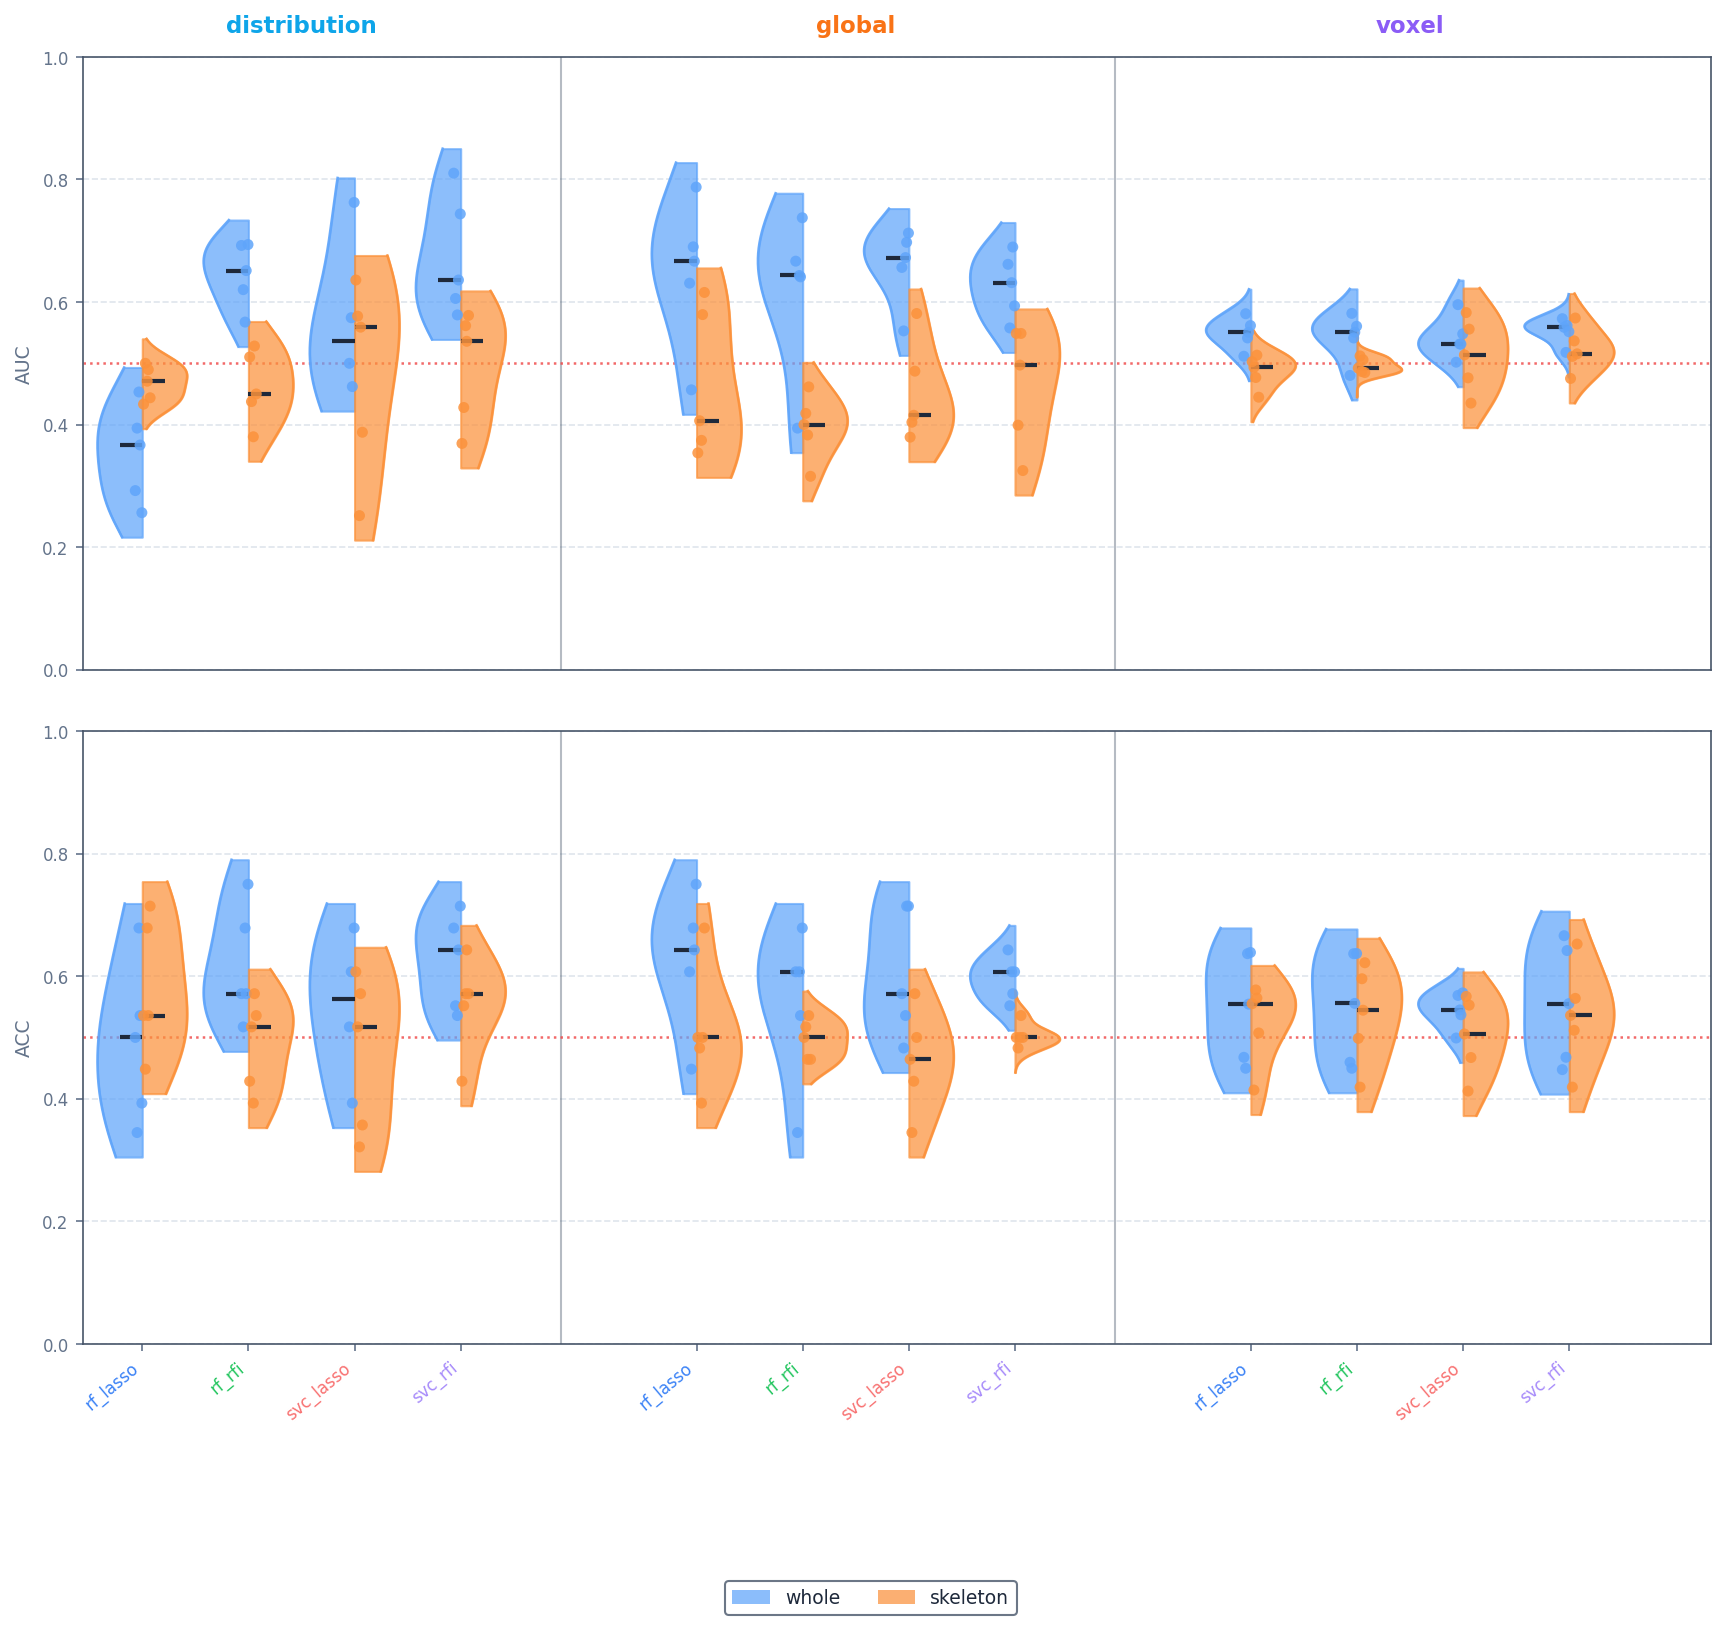
\includegraphics[width=1\textwidth]{doc/05_07_auc_acc_method_fset.png}
\caption{AUC (top) and ACC (bottom) distributions across all evaluated classifiers and feature sets. Results are grouped by feature set type: distribution-based, global-based, and voxel-based. Within each group, individual violin plots correspond to one classifier. The left half of each violin plot represents models trained on whole-thrombus features; the right half represents models trained on thrombus core features. RF: random forest classifier; SVC: support vector classifier; RFI: random forest importance-based selector; LASSO - least absolute shrinkage and selection operator selector.}\label{fig.AUC_ACC_distributions_all}
\end{figure}

As visible in Fig.~\ref{fig.AUC_ACC_distributions_all}, the meaningful performance of the models decreased when only the core voxels of the thrombus were selected compared to the results achieved using the information from the whole clot. Accordingly, even though the precision of the voxel based models was high, the voxel based dataset appeared to contain insufficient information to distinguish between SRP/nSRP and led to model underfitting with the prediction of the same label regardless of the method used. These results confirm the expected findings, that the information provided by a single voxel is insufficient to establish the clinical outcome. Nevertheless, this dataset was crucial for the creation of the global and distribution based datasets.

The investigation, whether the models performance is higher than  Based on the Fig.~\ref{fig.D3_cohens_kappa_heatmap_all_fsets} of the Cohen's~$\kappa$ comparing the performance of the model to its randomized variant. The performance of the random model variant was obtained by randomly shuffling labels 100 times to the testing dataset. The mean accuracy achieved on the dataset with not true labels is considered as the accuracy of the random model with the same architecture and parameters as the predictive one. 

\begin{figure}[!htb]
\centering
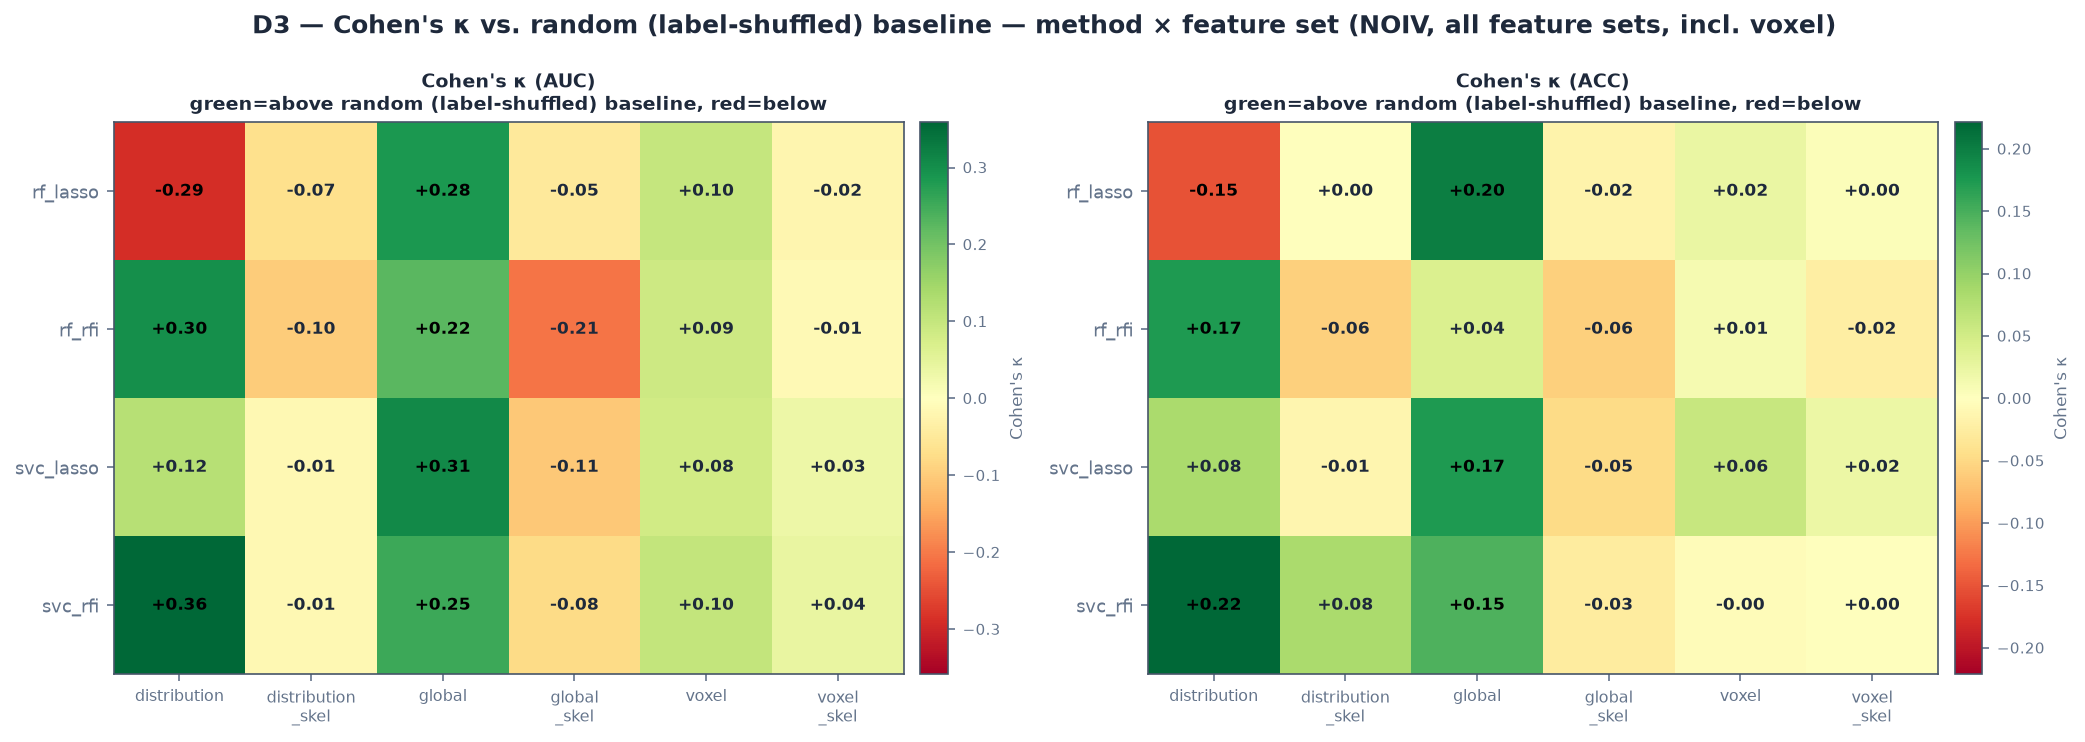
\includegraphics[width=1\textwidth]{doc/D3_cohens_kappa_heatmap_all_fsets.png}
\caption{Cohen§s Kappa  RF: random forest classifier; SVC: support vector classifier; RFI: random forest importance-based selector; LASSO - least absolute shrinkage and selection operator selector.}\label{fig.D3_cohens_kappa_heatmap_all_fsets}
\end{figure}



Due to the findings stated, further analysis will focus on the distribution and global based whole thrombus datasets. Results achieved using information only from the thrombus centerline and voxel-based dataset may be viewed in the supplementary material.  

The median AUC of the models using the global-based feature set was above 63\%, and the median ACC was higher than~57\%. These results substantially exceed the performance reported by~\cite{vanVoorst2022}, who achieved an AUC of~52\% for SRP prediction using only mean global thrombus radiomic features. 

In the case of the models using the distribution-based information, the median AUC of the LASSO-RF model achieved only~37\% and median ACC was~50\%. As visible in Fig.~\ref{fig.spline_combined_dist_global}, models using this method utilized only one feature for classifier training, when using the distribution-based dataset. Based on the results, the model was not able to fit appropriately during the entire optimization process, which resulted in a set of zero weighted coefficients for all provided features. Since all features were determined to be equally unimportant due to their low relationship with the SRP/nSRP, only the probability density in the first bin of the histogram created from the NCCT thrombus scan was selected for training. However, even though the median metric values of the rest of the classifiers reach almost the same fruitfulness as a random classifier, some models reach AUC and ACC above 70\%, which suggests that the distribution based features introduce clinically relevant information. 

\begin{figure}[!htb]
\centering
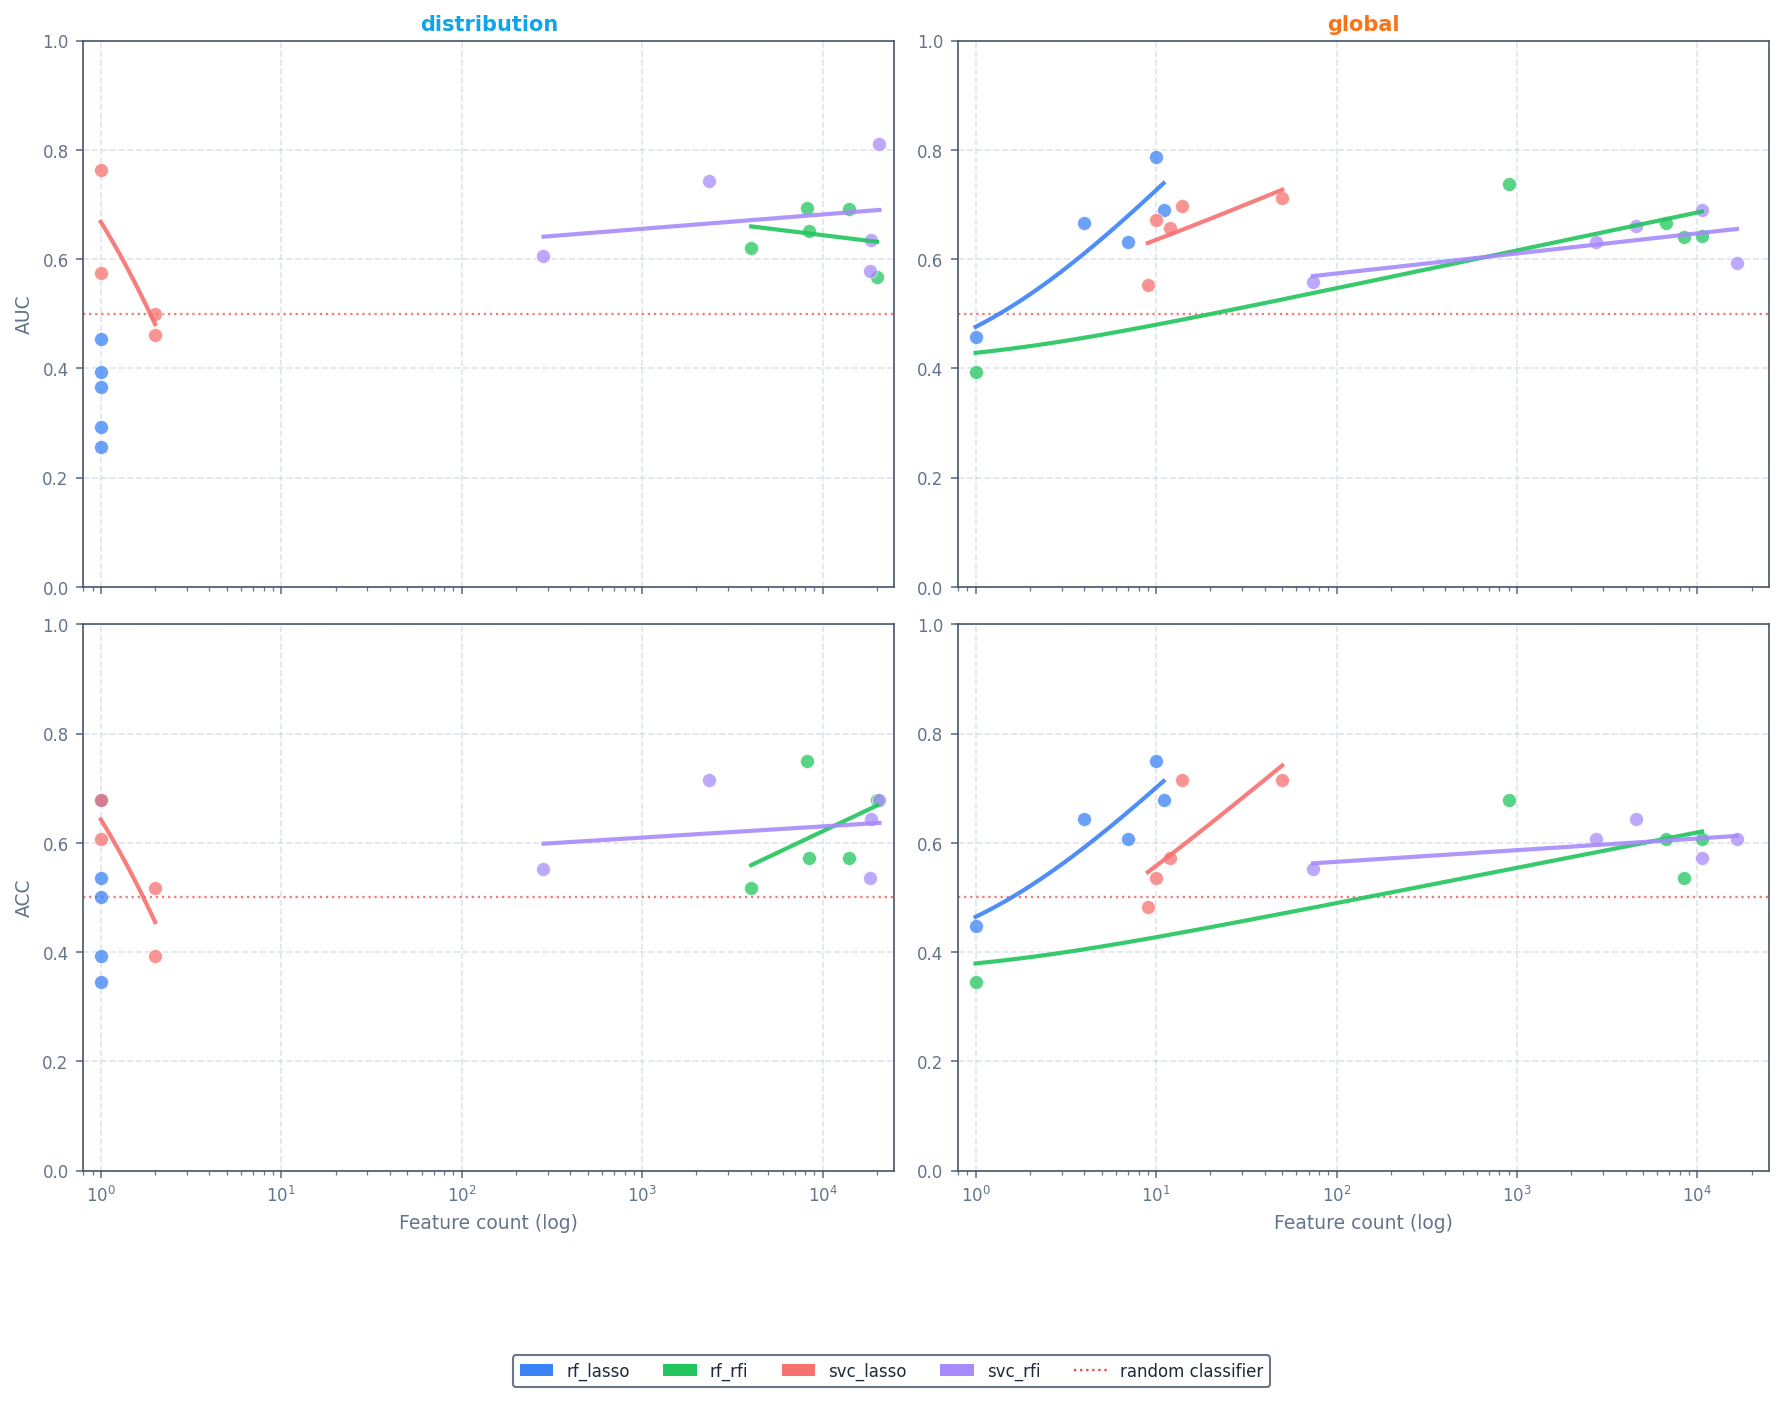
\includegraphics[width=1\textwidth]{doc/spline_combined_dist_global.png}
\caption{Dependence of the AUC (top) and ACC (bottom) on the number of selected features for models trained on whole-thrombus feature sets. Each point represents results achieved for a single split. Lines indicate linear regression trends fitted in log-space. RF: random forest classifier; SVC: support vector classifier; RFI: random forest importance-based selector; LASSO - least absolute shrinkage and selection operator selector.}\label{fig.spline_combined_dist_global}
\end{figure}

According to Fig.~\ref{fig.spline_combined_dist_global}, it is visible that models trained on the global-based dataset reached comparable or higher performance when selecting fewer than 100 out of 16528 features than those selecting more than 1000 features. Since models which used LASSO for feature selection achieve comparable AUC and ACC as the ones using RFI selector, the usage of these models is recommended as there is lower order of selected features, thus lower computational demand. 





\begin{figure}[!htb]
\centering
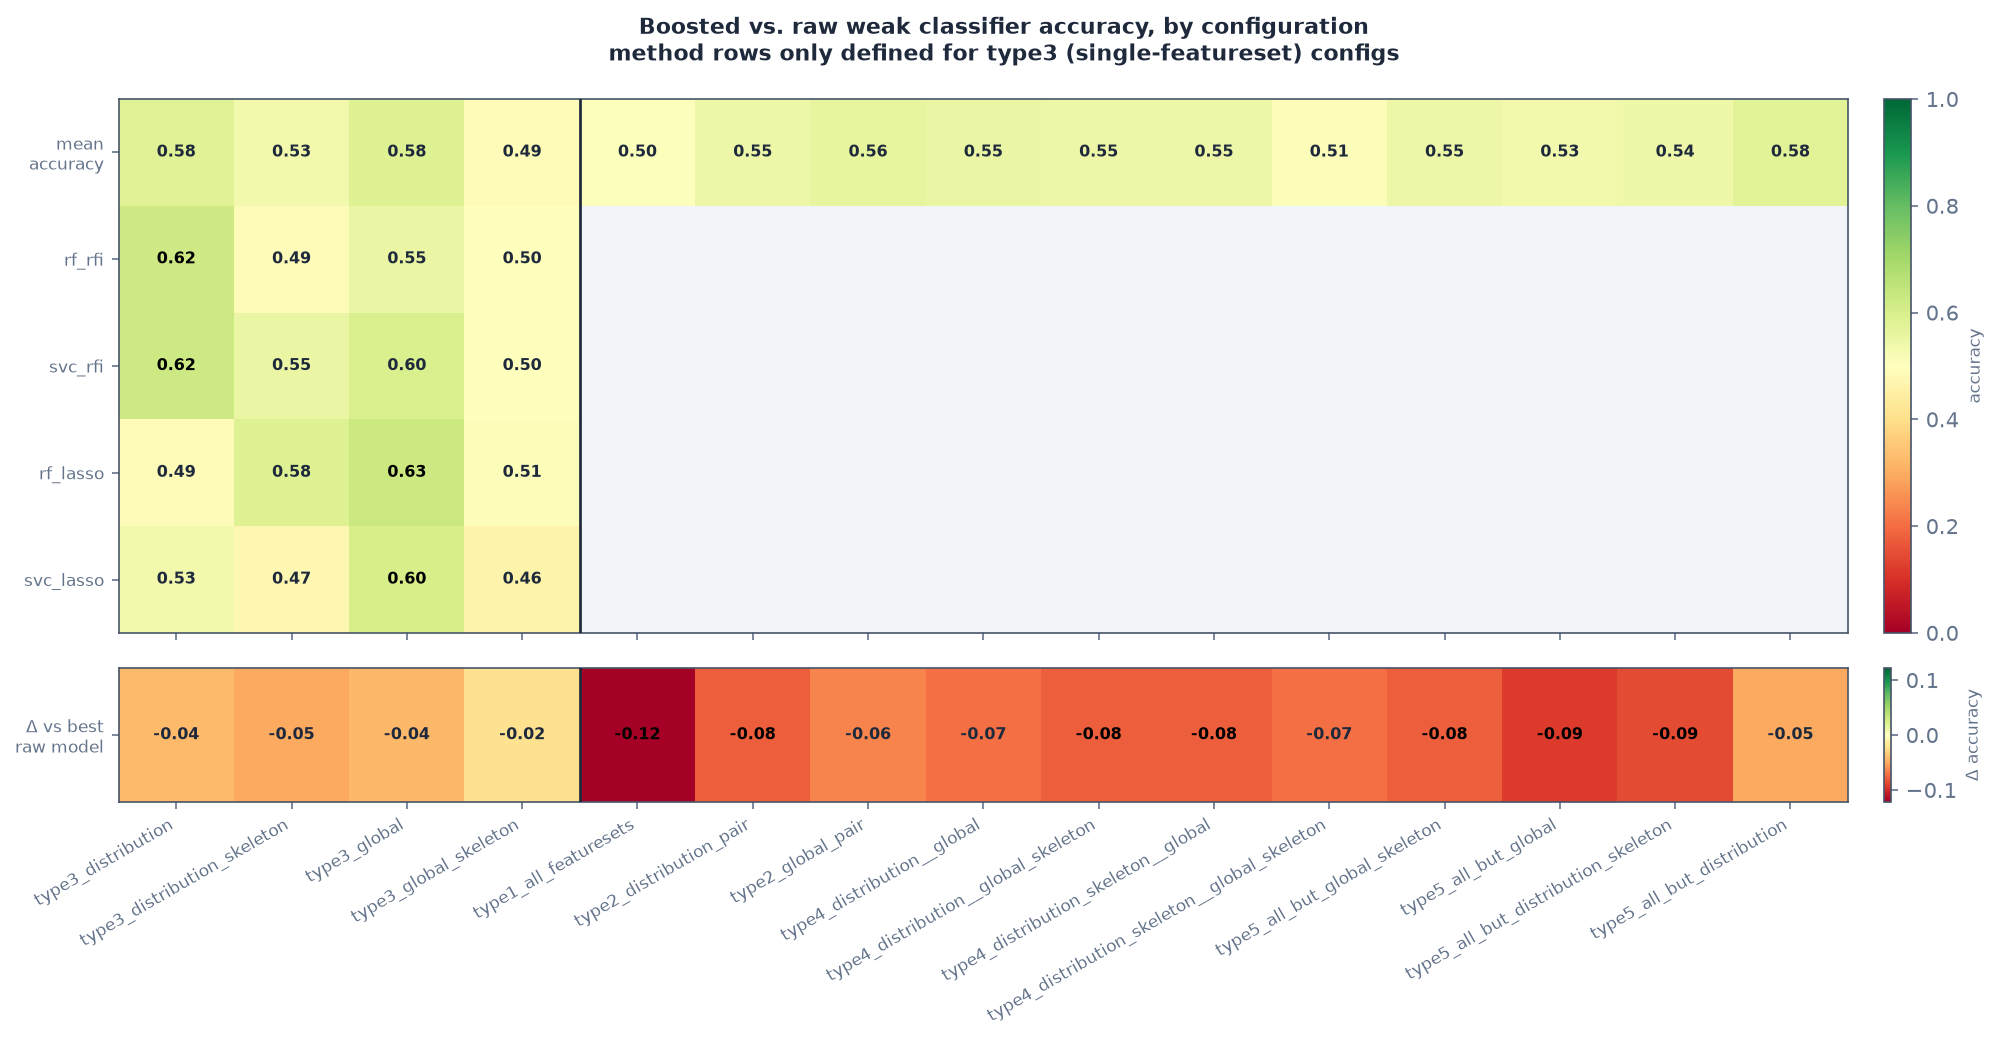
\includegraphics[width=1\textwidth]{doc/boosted_vs_raw_accuracy_heatmap.png}
\caption{ RF: random forest classifier; SVC: support vector classifier; RFI: random forest importance-based selector; LASSO - least absolute shrinkage and selection operator selector.}\label{fig.boosted_vs_raw_accuracy_heatmap}
\end{figure}

 


% major vote / most frequent prediction / confidence interval


Registry - different population, older scanners

\textbf{Limitations}






% \subsection{Example Subsection}
% \label{subsec1}

% Subsection text.

% %% Use \subsubsection, \paragraph, \subparagraph commands to 
% %% start 3rd, 4th and 5th level sections.
% %% Refer following link for more details.
% %% https://en.wikibooks.org/wiki/LaTeX/Document_Structure#Sectioning_commands

% \subsubsection{Mathematics}
% %% Inline mathematics is tagged between $ symbols.
% This is an example for the symbol $\alpha$ tagged as inline mathematics.

% %% Displayed equations can be tagged using various environments. 
% %% Single line equations can be tagged using the equation environment.
% \begin{equation}
% f(x) = (x+a)(x+b)
% \end{equation}

% %% Unnumbered equations are tagged using starred versions of the environment.
% %% amsmath package needs to be loaded for the starred version of equation environment.
% \begin{equation*}
% f(x) = (x+a)(x+b)
% \end{equation*}

% %% align or eqnarray environments can be used for multi line equations.
% %% & is used to mark alignment points in equations.
% %% \\ is used to end a row in a multiline equation.
% \begin{align}
%  f(x) &= (x+a)(x+b) \\
%       &= x^2 + (a+b)x + ab
% \end{align}

% \begin{eqnarray}
%  f(x) &=& (x+a)(x+b) \nonumber\\ %% If equation numbering is not needed for a row use \nonumber.
%       &=& x^2 + (a+b)x + ab
% \end{eqnarray}

% %% Unnumbered versions of align and eqnarray
% \begin{align*}
%  f(x) &= (x+a)(x+b) \\
%       &= x^2 + (a+b)x + ab
% \end{align*}

% \begin{eqnarray*}
%  f(x)&=& (x+a)(x+b) \\
%      &=& x^2 + (a+b)x + ab
% \end{eqnarray*}

% %% Refer following link for more details.
% %% https://en.wikibooks.org/wiki/LaTeX/Mathematics
% %% https://en.wikibooks.org/wiki/LaTeX/Advanced_Mathematics

% %% Use a table environment to create tables.
% %% Refer following link for more details.
% %% https://en.wikibooks.org/wiki/LaTeX/Tables
% \begin{table}[t]%% placement specifier
% %% Use tabular environment to tag the tabular data.
% %% https://en.wikibooks.org/wiki/LaTeX/Tables#The_tabular_environment
% \centering%% For centre alignment of tabular.
% \begin{tabular}{l c r}%% Table column specifiers
% %% Tabular cells are separated by &
%   1 & 2 & 3 \\ %% A tabular row ends with \\
%   4 & 5 & 6 \\
%   7 & 8 & 9 \\
% \end{tabular}
% %% Use \caption command for table caption and label.
% \caption{Table Caption}\label{fig1}
% \end{table}


% %% Use figure environment to create figures
% %% Refer following link for more details.
% %% https://en.wikibooks.org/wiki/LaTeX/Floats,_Figures_and_Captions
% \begin{figure}[t]%% placement specifier
% %% Use \includegraphics command to insert graphic files. Place graphics files in 
% %% working directory.
% \centering%% For centre alignment of image.
% \includegraphics{example-image-a}
% %% Use \caption command for figure caption and label.
% \caption{Figure Caption}\label{fig1}
% %% https://en.wikibooks.org/wiki/LaTeX/Importing_Graphics#Importing_external_graphics
% \end{figure}


% %% The Appendices part is started with the command \appendix;
% %% appendix sections are then done as normal sections
% \appendix
% \section{Example Appendix Section}
% \label{app1}

% Appendix text.

% %% For citations use: 
% %%       \cite{<label>} ==> [1]

% %%
% Example citation, See \cite{lamport94}.

%% If you have bib database file and want bibtex to generate the
%% bibitems, please use
%%
\bibliographystyle{elsarticle-num} 
\bibliography{BibFile}

%% else use the following coding to input the bibitems directly in the
%% TeX file.

%% Refer following link for more details about bibliography and citations.
%% https://en.wikibooks.org/wiki/LaTeX/Bibliography_Management


\end{document}

\endinput
%%
% %% End of file `elsarticle-template-num.tex'.
